\documentclass[10pt]{article}
\usepackage[left=20mm,right=20mm,top=25mm,bottom=25mm]{geometry}
\usepackage{amsmath} % math
\usepackage{amssymb} % math
\usepackage{graphicx} % to use \includegraphics{}
\usepackage{diagbox} % to make tables
\usepackage{multirow}
\usepackage[labelsep=period]{caption}
\usepackage{subcaption}
\usepackage[hangul]{kotex}
\usepackage{color}
\usepackage[hidelinks]{hyperref}
\usepackage[per-mode=symbol]{siunitx}
\sisetup{inter-unit-product =$\cdot$} % http://tex.stackexchange.com/questions/59032/how-to-format-si-units
%\graphicspath{{images/}}
\usepackage[T1]{fontenc}   % To use Times New Roman
\usepackage[utf8]{inputenc}% To use Times New Roman
\usepackage{mathptmx}      % To use Times New Roman
\usepackage{titlesec}
\usepackage{lipsum} % Lorem Ipsum ㅁㄴㅇㄹ 

%%%%%% Section Title Setting %%%%%%% 
\titleformat*{\section}{\fontsize{12}{12}\selectfont\bfseries}
\titleformat*{\subsection}{\fontsize{11}{11}\selectfont}
\titleformat*{\subsubsection}{\normalfont}
\def\thesection{\Roman{section}.}
\def\thesubsection{\arabic{subsection}.}
\def\thesubsubsection{\normalfont \arabic{subsection}.\arabic{subsubsection}.}
\makeatletter
\renewcommand{\@seccntformat}[1]{\csname the#1\endcsname\ }
\makeatother

%%%%% Caption(Figure/Table) Setting %%%%%%%
\captionsetup{figurename=Fig.} % Figure label (FIG: --> FIGURE)
\captionsetup[table]{
	name=Table,   % Table label (Table --> TABLE)
	singlelinecheck=off  % Left aligned
}


\begin{document}
\begin{center}
	\fontsize{16pt}{16pt}\selectfont{\bf R\&E 과제명(국문)}\\
	\fontsize{10pt}{10pt}\selectfont{ 저자명 \textperiodcentered  저자명 \\}
	\fontsize{10pt}{10pt}\selectfont{ 경기과학고등학교 \\}
	\vspace{0.6cm}
	\fontsize{16pt}{16pt}\selectfont{\bf Title(English) \\}
	\fontsize{10pt}{10pt}\selectfont{ author name \textperiodcentered  author name \\}
	\fontsize{10pt}{10pt}\selectfont{ Gyeonggi Science High School \\}
	\vspace{1cm}
	\fontsize{12pt}{12pt}\selectfont{\bf 국문 초록 \\}
\end{center}
\begin{table}[h]
	\begin{tabular}{p{\textwidth}}
		\hline
		국문 초록은 400자 내외로 작성한다.  
		
		주제어: 주제어, 예시, 주제어 예시(5개 이내)
		\hline
	\end{tabular}
\end{table}
\section{서론}
청소년 과학창의연구 학술지 \footnote{각주 예시}는 과학(예술)영재학교 및 과학고등학교의 재학생이면 누구나 투고할 수 있는 학술지이다 \cite{song}.
\section{이론적 배경}
\subsection{소제목}
\subsubsection{과학영재 창의연구(R\&E)}
\lipsum[1]
\begin{table}[h]
	\centering
	\caption{홀수 짝수}
	\label{oddeven}
	\begin{tabular}{|c||c|c|c|}
		\hline
		may have P.P & -했을지도 모른다 & 과거의 약한 추측 & $\fallingdotseq$ might have P.P\\
		\hline
		can have P.P & -할 수 있었을 것이다 & 과거의 가능성 & \\
		\hline
		would have P.P & -했을 것이다 & 과거의 의지 & \\
		\hline
		must have P.P & -했음에 틀림없다 & 과거의 강한 추측 & \\
		\hline
		should have P.P & -했어야 한다 & 과거의 유감 & $\longleftrightarrow$ should not have P.P \\
		\hline
		cannot have P.P & -했을리가 없다 & 과거의 강한 부정추측 & \\
		\hline
	\end{tabular}
\end{table}
\section{연구 방법 및 절차}
\lipsum[2]
\begin{figure}
	\centering
	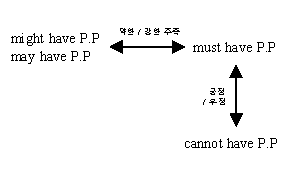
\includegraphics[width=0.6\textwidth]{modal.pdf}
	\caption{Modal verbs}
	\label{modal_verbs}
\end{figure}
\begin{thebibliography}{00}
	\bibitem{song}{송경애 (2005). 중학생 영재의 비지적특성과 가정의 과정변인이 수학적 창의성에 미치는 영향. 박사학위논문. 건국대학교.}
\end{thebibliography}
\end{document}
